\documentclass[conference]{IEEEtran}
%\documentclass{ieeeconf} 

%\IEEEoverridecommandlockouts    %Needed if you want to use the \thanks command

%\overrideIEEEmargins %Needed to meet printer requirements.

%\usepackage[lined,ruled]{algorithm2e}
%\usepackage{geometry}
\usepackage{amssymb,amsmath}
\usepackage{graphicx}
\usepackage[usenames,dvipsnames]{pstricks}
\usepackage{epsfig}
\usepackage{booktabs}
\usepackage{pst-grad} % For gradients
\usepackage{pst-plot} % For axes
\usepackage{url}

\newcommand{\eat}[1]{}

%\geometry{top=1.0in, bottom=1.0in, left=0.7in, right=0.7in}
\topmargin = -1.5cm
\textheight = 24cm

\title{Exploiting Data Parallelism in SELinux using a Multi-core Processor}


\author{
    \IEEEauthorblockN{Arun Kalyanasundaram\IEEEauthorrefmark{1}\IEEEauthorrefmark{3},
      Bodhisatta Barman Roy\IEEEauthorrefmark{2}\IEEEauthorrefmark{5}, Shrisha Rao\IEEEauthorrefmark{1}\IEEEauthorrefmark{4}}
    \IEEEauthorblockA{\IEEEauthorrefmark{1}International Institute of
      Information Technology Bangalore, India
    \\\IEEEauthorrefmark{3}arun.k@iiitb.net, \IEEEauthorrefmark{4}shrao@ieee.org}
    \IEEEauthorblockA{\IEEEauthorrefmark{2}National University of
      Singapore, Singapore
    \\\IEEEauthorrefmark{5}bodhi@comp.nus.edu.sg}
}



% \author{Arun Kalyanasundaram and Bodhisatta Barman Roy and Shrisha Rao\\% <-this % stops a space
% International Institute of Information Technology\\
% Bangalore, India
% }

%****The document begins here****

\pagestyle{empty}


\begin{document}

\maketitle
\begin{abstract}

Security Enhanced Linux, popularly known as SELinux \cite{s1} is a 
Linux operating system feature that provides fine grained access 
control to system resources. Our goal is to optimize the performance of SELinux for a multi-core processor and analyze the potency of our approach. We study the architecture of SELinux to identify specific components that cause performance bottlenecks and empirically validate our claims. We propose various techniques to delegate processor intensive computations to multiple cores. We perform several experiments to evaluate the performance of our approach under different conditions and discuss the intricacies of our implementation. 
Our results show that software applications with security validations, in general have an inherent data parallelism which can be exploited for concurrent execution, but
  the gain in efficiency depends on design of the application and the
  hardware platform. In addition, we find that the gain in efficiency is also influenced by the optimization technique and the system configuration.   We use a Cell
  Broadband Engine (CBE) processor running SELinux for our experiments, but
  our approach can be easily adapted to applications with a similar
  security validation framework running on other multi-core platforms.
\end{abstract}

{\bf Keywords:} Parallel Algorithms, Security, Operating Systems,
Security Enhanced Linux, Cell Broadband Engine

\thispagestyle{empty}

%******First section for intro******

%
%----------The bibliography-------
% 
\section{Introduction}\label{intro}
SELinux is a Linux operating system feature that implements the
Mandatory Access Control (MAC) security paradigm. MAC operates on a
set of rules to constrain a `process' from performing a particular
operation on a resource (e.g. file, directory, etc). These rules form the
security policy of a system and is centrally controlled by an
administrator. Each resource and process is assigned a
label called the \emph{security context} (SC). Thus a rule simply
states if one SC is allowed to perform an operation on another SC.

One of the major drawbacks of SELinux is the performance overhead associated with it. The system performance reduces by about 7\% when SELinux is enabled and in certain cases like networked systems, the
overhead may be much higher \cite{selinuxFAQ}. In addition, the worst
case performance could be unacceptably low depending on the number of
rules in the security policy \cite{report}. Our goal is to optimize the performance of SELinux for a multi-core processor and analyze the effectiveness of our approach.

In this paper, we first study the architecture of SELinux to determine
the scope for introducing data parallelism. We pin-point
the specific components within SELinux that cause performance
bottlenecks and empirically validate our claims. Based on our analysis, we propose various techniques
to modify the SELinux architecture for parallel
execution. Our work takes a high level approach so that our proposed techniques can also be applied to other large scale security software. More specifically, we optimize the general process of security validations which involves verifying the credibility of a given entity against a set of trusted entities. We
perform several experiments to evaluate the performance of our approach under different conditions. For our experiments, we use the Cell Broad Engine (CBE) multi-core processor since it is
known to outperform existing processors by almost an order of magnitude \cite{CBEArch}. 

%Sections organized
The rest of the paper is organized as follows. In Section \ref{background}, we discuss the background and state of art related to our work. In Section \ref{design}, we
study the architecture of SELinux to identify performance bottlenecks and propose various techniques to
achieve data parallelism. In Section \ref{expr}, we discuss our experimental setup, intricacies / challenges of our implementation, results and inferences. We conclude with scope for future work in
Section \ref{conclusion}.

\section{Background and Related Work}\label{background}

Security has been an integral part of every software
application and a primary focus of Networking and Operating Systems research. 
With the advent of cloud computing,
security has gained prominence like never before, since these
applications can now be accessible from anywhere in the world and thus
are more vulnerable than their stand-alone counterparts. However,
security comes with a steep price in the form of loss in efficiency. But when it comes to building a security feature, efficiency is generally given less importance over robustness. This trend has led to significant performance loss in modern day systems, where even an
anti-virus application can slow down the system by more than fifty
percent. This applies even to operating systems' inbuilt security
features like SELinux \cite{s1}, RSBAC \cite{s2}, TOMOYO 
Linux\footnote{http://tomoyo.sourceforge.jp}, AppArmor\footnote{http://wiki.apparmor.net}.

With processor clock speed reaching a saturation, extensive research is underway in optimizing existing software applications for multi-core processors. Our work aims to exploit data parallelism in SELinux to optimize its performance for multi-core processors. There has not been any size-able effort in optimizing the performance
of SELinux \cite{selinuxFAQ}. Although there has been some work on
optimizing SELinux for 32 or more processors, but no further details
exist \cite{selinuxFAQ}. There have been attempts to extend the SELinux functionality to a distributed setting \cite{tresys}.  Brindle, et al. \cite{tresys} present a distributed policy
management architecture and address several challenges like
synchronization of policy updates, managing multi-system policy,
etc. In this paper, we focus on optimizing SELinux for a single system
with multiple processors (or cores), rather than an inter-connected distributed
system, which could be a scope for future work. The multi-core optimization is also based on implementing parallelized data-structures \cite{ll1}.

SELinux is based on the Flux Advanced Security Kernel (Flask)
architecture \cite{flask}. It consists of two major components, the
\emph{Object Manager} which enforces security policy decisions and the
\emph{Security Server} which provides security decisions. The \emph{Object
Manager} is responsible for labeling the resources and respond to
changes in the security policy \cite{flask}. Every access permission
request has to be authorized by the \emph{Object Manager}, and these requests
are managed by the Linux Security Module (LSM) framework
\cite{selinuxBook}. LSM consists of a set of hooks at specific points
in the kernel where access to a resource is from a system call. These
hooks are a set of function pointers which by default do nothing,
unless overridden by a security module like SELinux. The return values
of these hooks determine whether an access is granted or denied.

When the \emph{Object Manager} receives a request from LSM, it
extracts the security context of the source and target, to invoke the
\emph{Security Server} with these parameters. The \emph{Security Server} makes the
decision to grant / deny the requested operation based on the rules
specified in the security policy. The\emph{Object Manager} maintains a
history of such access decisions in a data structure called the Access
Vector Cache (AVC). The AVC helps to optimize future requests, since
the decision making logic of the security server is extremely
processor-intensive. The AVC is a simple hash-table implementation
using 128 buckets with open addressing. The size of AVC is
configurable, however a maximum of 512 entries is found to be optimal
in order to maintain a smaller chain length \cite{selinuxBook}. Hence,
the \emph{Object Manager} can bypass the \emph{Security Server} when a requested
access decision is available in the AVC.

We evaluate the performance of SELinux using a Cell Broadband Engine (CBE) multi-core processor which consists of one Power Processing
Element (PPE) and eight Synergistic Processing Elements (SPE)
\cite{CBEArch}.  The SPEs are designed specifically to perform
processor intensive computations. A SPE by itself can not initiate a
computation, only a PPE can initialize an SPE by loading the desired
executable binary into the SPEs' local cache. In addition, data
required by an SPE during execution requires the use of Direct Memory
Access (DMA) controllers. At the time of SPE initialization, the PPE
sends an address of a location in main memory which the SPE can use as
a base address to read / write data. In order to access contents of
the main memory, the SPE makes a DMA request with the base address,
the number of bytes and the type of access (read or write). Each SPE
has one or more dedicated DMA engines that perform data transfers to
and from main memory to SPEs' local cache, in concurrent with program
execution. In our implementation we use the CBE SDK which provides
flexible APIs which can perform both asynchronous and synchronous DMA
requests.

Performing large scale experiments using SELinux requires the creation of several security
policies with different configurations. But creation of policies is a
hard and tedious process. In general, it is a job of system
administrators to write these policies which typically contain
thousands of rules. Another issue with manual maintenance of large security
policies is the detection of loopholes which could lead to possible
security breach. Several tools have been developed to automate the
process of SELinux policy configuration \cite{selinuxTools}. While
these tools mainly provide effective analysis of security policies
\cite{selinuxTools}, policy creation is still a manual
process. Therefore, we
implement a set of Unix shell-scripts to
automatically generate SELinux security policies with a specific access permission
pattern
\footnote{http://selinuxoncbe.svn.sourceforge.net/viewvc/selinuxoncbe/trunk/src/policies/scripts/}.


\section{Design}\label{design}

In SELinux access control, a process can perform an operation
(e.g. read, write etc.) on a resource (e.g. files, directories, ports, etc.)
only when the corresponding rule is specified in the policy. A rule
simply states if a security context can perform a particular operation
on another security context. Each process and resource on the system
is associated with a security context, and the decision to allow or
disallow an operation is based on the following,

\begin{itemize}

\item The validity of the security contexts of source (process) and target (resource).
\item The presence of a rule in the policy that allows the requested operation. 

\end{itemize}

A security context is considered valid if each of its three components
(user, role and type) are valid. The validation is performed by
extracting each component and matching it against a \emph{list of
  valid contexts}. We will show in Section \ref{results} that the
validation step is the major cause for performance overhead of
SELinux. We therefore model this step for parallel execution using the
SIMD (Single Instruction Multiple Dataset) programming
paradigm. Specifically, we look at exploiting data parallelism by
dedicating one or more processing units to the matching operation of
each component of security context. We use the principle of SIMD
because each processing unit operates on a different data, but execute
the same set of instructions. Since the security context has three
components, we can use a minimum of three processing units considering
each component requires one dedicated unit. We propose the following
techniques based on the number of processing units and its loading
strategy, and compare their relative performances (runtime).

\begin{itemize}

\item \textbf{Three Processing Units ($3U$)}: In this technique we use
  one dedicated processing unit to for each component of the security
  context, hence a total of three units. In the Cell Broadband Engine
  processor, these processing units are the Synergistic Processing
  Elements (SPEs), which operate in slave mode (Section
  \ref{background}). Each SPE performs a linear search on the list of
  valid contexts corresponding to each component of the security
  context as shown in Figure \ref{figOneSPE}. The dashed line in
  Figure \ref{figOneSPE} shows the direction of traversal.

\item \textbf{Three Processing Units with Busy Wait ($3UBW$)}: In
  general, SPEs are initialized with a set of instructions and a base
  address of the required data in main memory. To access this data,
  the SPE has to make DMA requests and wait until the data is received
  (Section \ref{background}). However, when the data is not stored in
  consecutive chunks of memory (e.g. linked list), the SPE is
  initialized every time with the address of the next chunk of data,
  which is the approach we use in $3U$ (mentioned above). But we
  observed that the frequent initialization of SPE has a significant
  performance overhead. Therefore we devise a busy wait technique, in
  which the SPE is initialized with the address of a unique location
  in main memory\eat{ instead of the base address of the data}. This
  location is updated with the base address of the next chunk of data,
  every time after the SPE reads it. The details of the implementation
  are given in Section \ref{impl}.

\item \textbf{Six Processing Units ($6U$)}: This technique is similar
  to $3U$, except that two dedicated SPEs per component of the
  security context are used instead of just one. Thus a total of six
  processing units are used in this technique. Since two SPEs operate
  on the list simultaneously, each SPE can process either the odd or
  even numbered elements of the list as shown in Figure
  \ref{figTwoSPE}.

\item \textbf{Six Processing Units with Busy Wait ($6UBW$)}: In this
  we use six processing units using the same design as given in $6U$,
  with each SPE operating in the busy wait mode as described in
  $3UBW$.

\end{itemize}

\begin{figure}
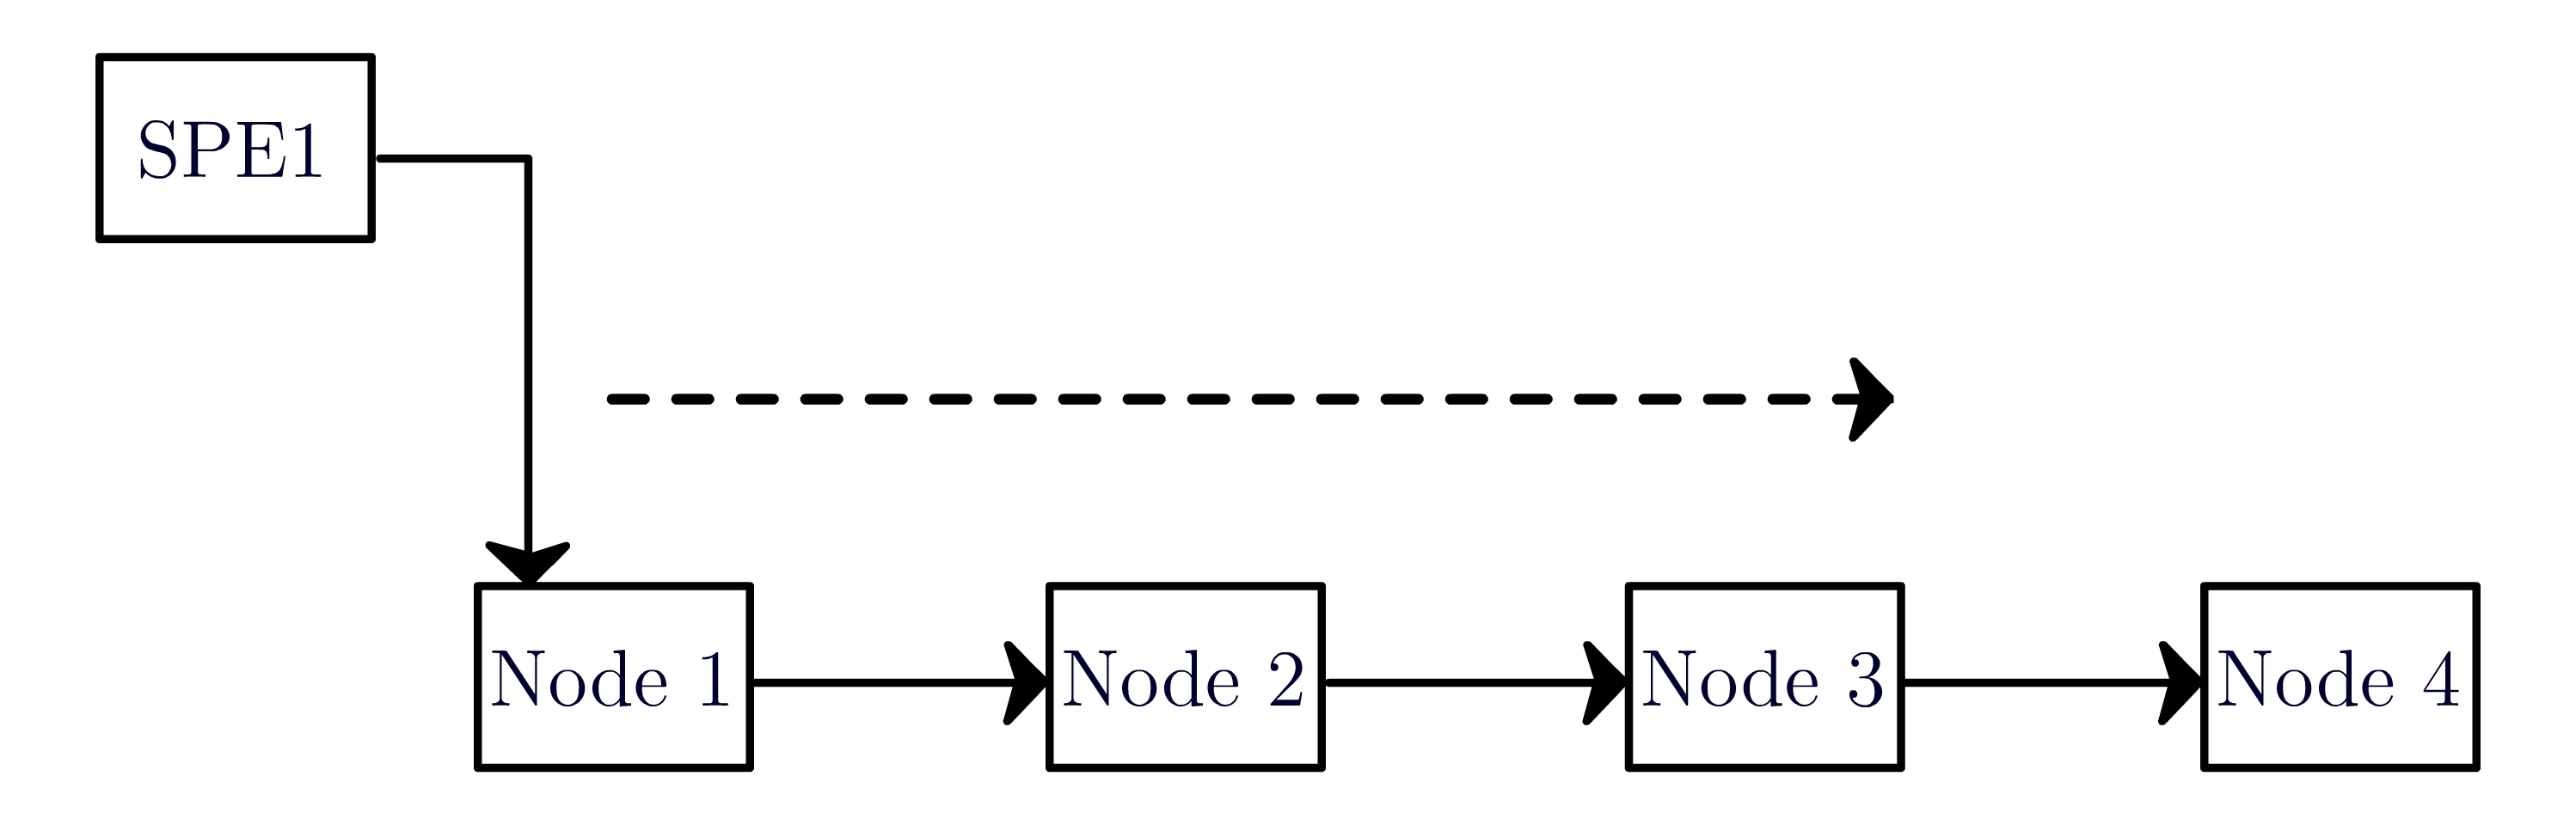
\includegraphics[scale=0.45]{images/oneSPE.png}
\caption{Traversing a linked list using one SPE.}
\label{figOneSPE}
\vspace{0.05cm}
\end{figure}


\begin{figure}
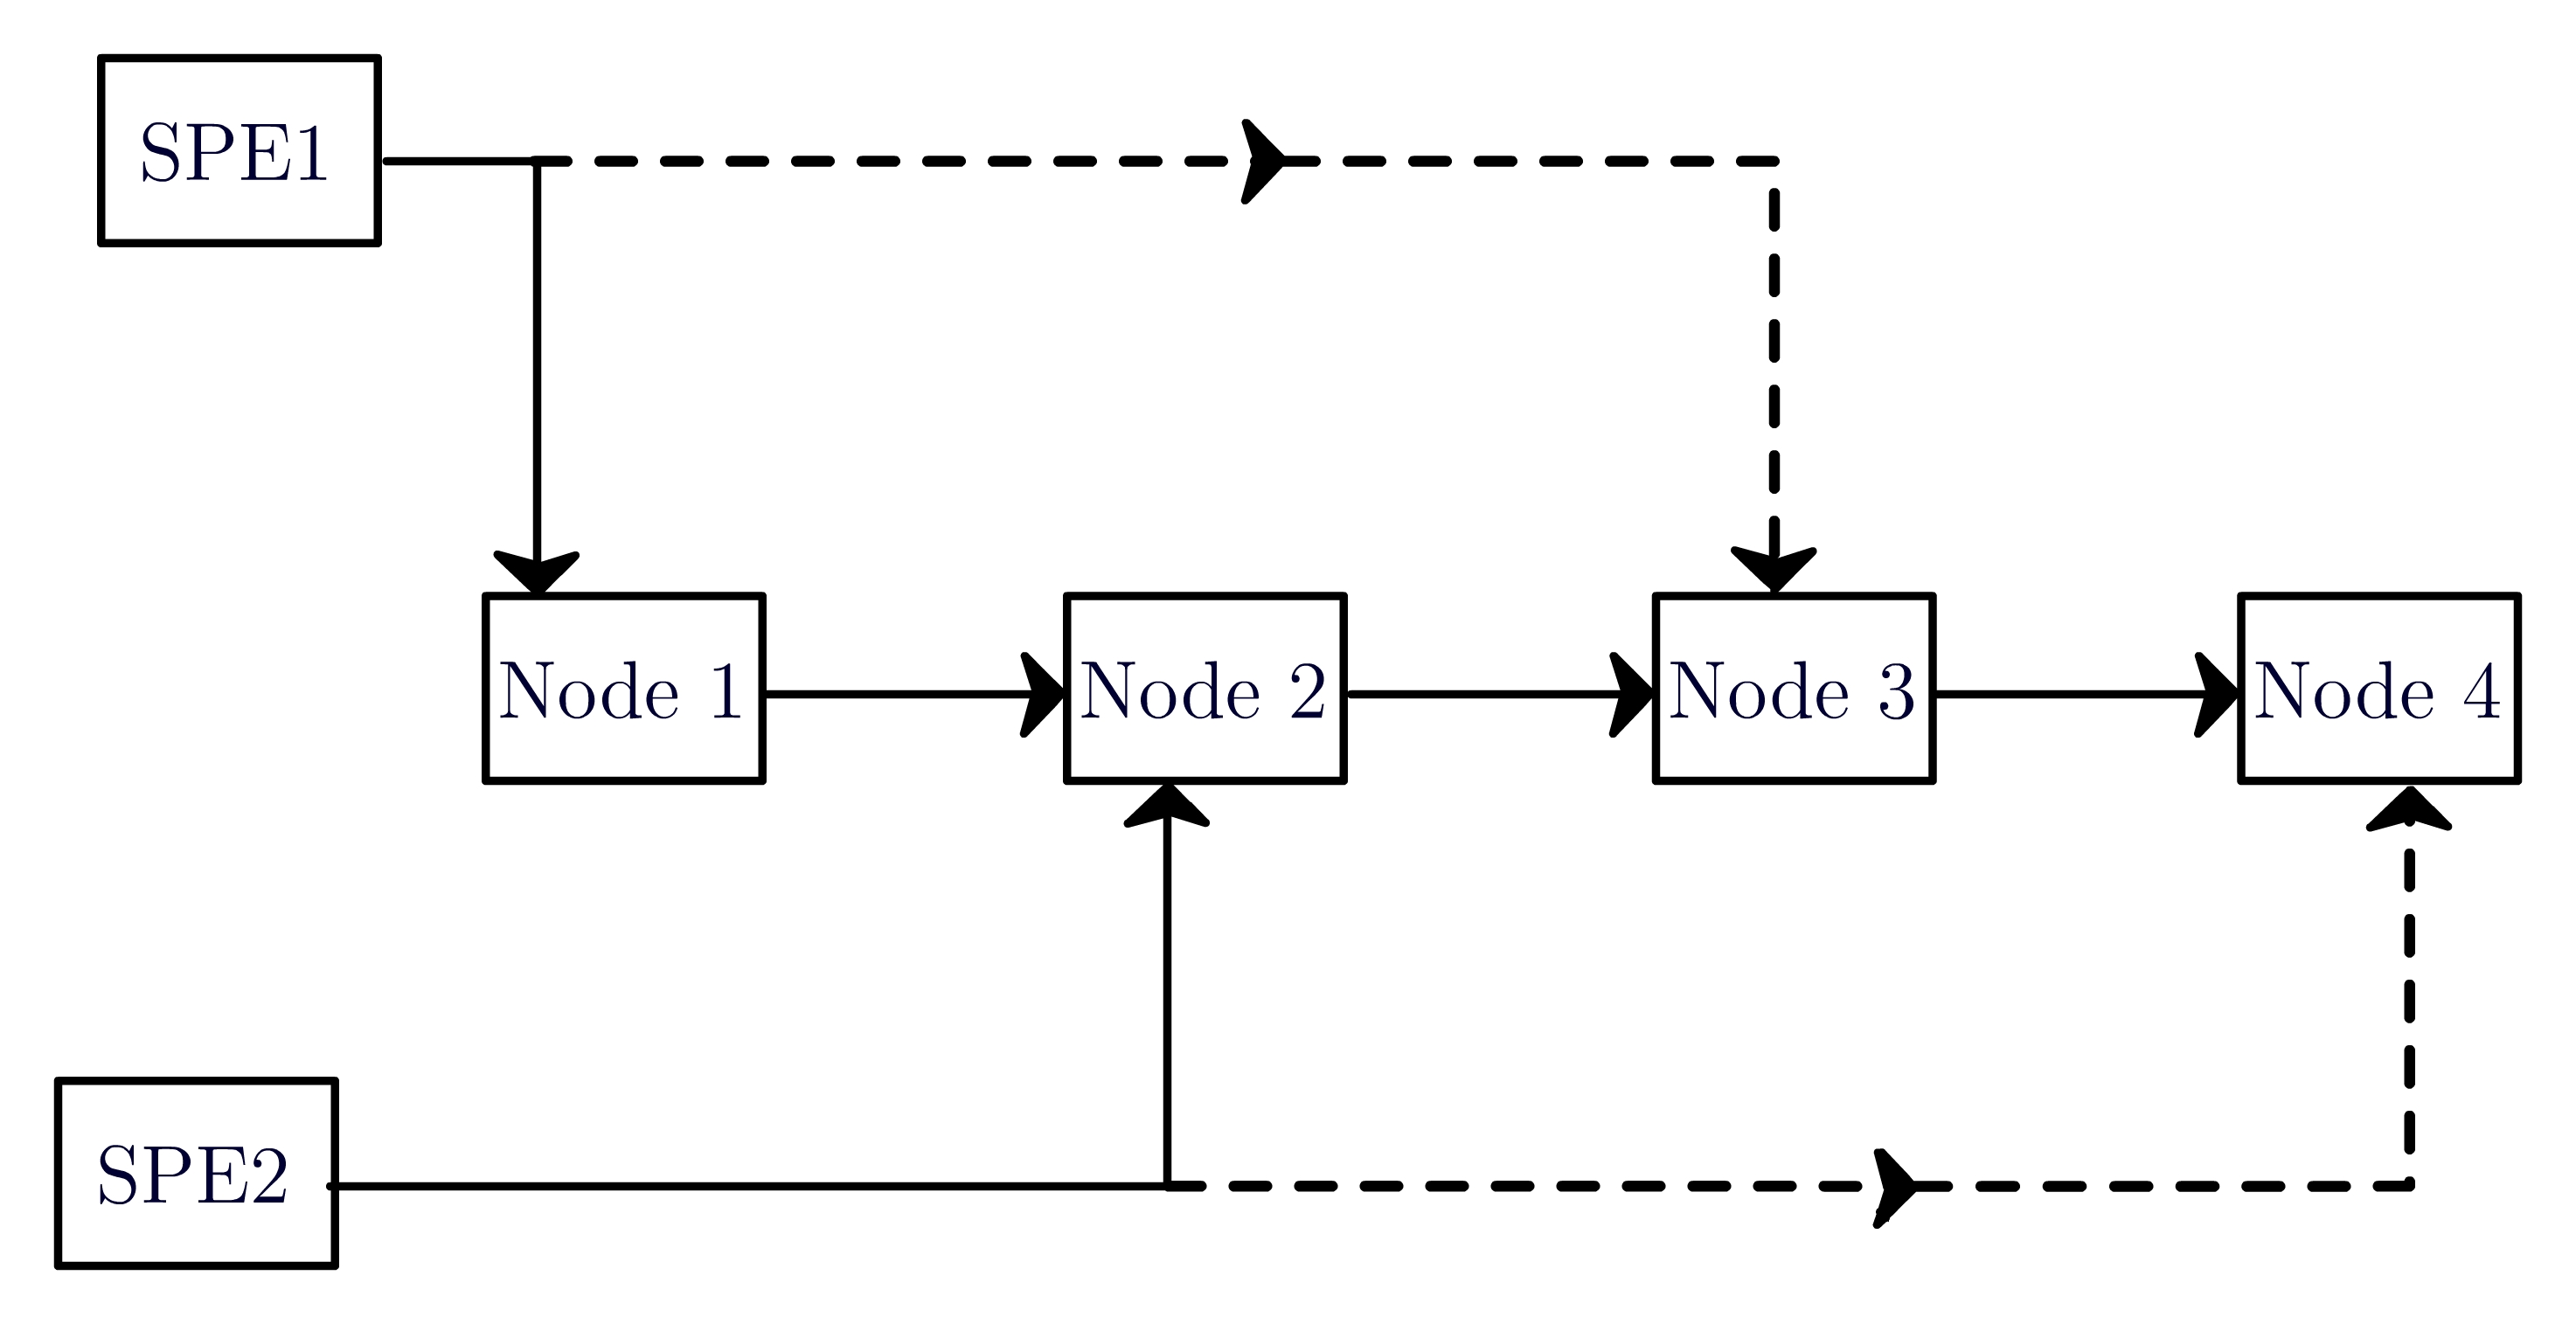
\includegraphics[scale=0.45]{images/twoSPE.png}
\caption{Traversing a linked list using two SPEs.}
\label{figTwoSPE}
\vspace{0.05cm}
\end{figure}

\section{Experiments}\label{expr}

The goal of our experiments is to evaluate the performance of different techniques proposed in
Section \ref{design}, on a CBE processor. For this purpose we use the
\emph{Sony Play Station 3} (PS3) with \emph{Yellow Dog Linux 6.1} (for
PowerPC architecture) installed. The PS3 has eight SPEs, out of which
six are accessible to a programmer. SELinux is a part of the security module of the
mainline Linux kernel since version 2.6. However the default installation of YDL does not contain
SELinux. Therefore in our setup, we recompile the Linux kernel (version 2.6.27) for the PowerPC architecture 
with the necessary configurations (file-system extended attribute support, security hooks, etc.) to enable SELinux \cite{report}. 

We use our experimental setup to study the impact of the following two configurable parameters - 1) number of valid security contexts and 2) size of Access Vector Cache (AVC). The number of valid
security contexts is determined by the number of rules in the policy
configuration file. The size of AVC, plays an important role in the performance of SElinux (Section \ref{background}), hence we evaluate
the performance both in the presence and absence of AVC. For
simplicity, we run our experiments with two different sizes of AVC -
512 and 1, which allows us to effectively quantify the performance of
security context validation with and without AVC respectively. A maximum size of 512 entries in AVC has been found to be optimal in order to maintain smaller chain lengths \cite{selinuxBook}.

Broadly, our experiments can be divided into two phases. In the first phase, we evaluate the performance of SELinux using only the single core (PPE) of the CBE processor. This involves measuring the performance with different number of rules in the policy configuration file. We will use this to establish a performance benchmark and to show that the security context validation step is indeed highly processor intensive. In the second phase, we compare the performance of the SIMD techniques proposed in Section \ref{design} with the single core performance. In each phase the experiments are performed with the presence and absence of AVC. 

\subsection{Implementation Details}\label{impl}

%Since the CBE SDK (version 3.1) does not support kernel space libraries, we perform our experiments using only the SELinux user space libraries.
In SELinux, the process of associating a security context to a resource on the file system is called \emph{labeling}. When the system boots
with SELinux enabled, the labeling of the file system takes place based on the settings
in $file\textunderscore contexts$ \cite{selinuxBook}. Once labeled, the security context cannot be changed without authorization. However,
malicious programs can sometimes take advantage of weak policy
configurations to modify the security contexts of certain files. This
could be a significant security breach and may allow undesirable
processes to access protected files. Therefore, SELinux provides a functionality to re-label the file-system, which allows to restore the original security context on system resources without having to reboot the system. The re-labeling process validates the security context of the resource being labeled against a list of valid contexts. This is the same operation that is performed by the security server of SELinux to make access decisions. Hence in our experiments we evaluate the performance of this re-labeling process to capture the overhead due to security validations in SELinux. The SELinux user-space libraries (\emph{setfiles}, \emph{libselinux} and \emph{libselpol}) are modified appropriately to incorporate the proposed SIMD techniques. In addition, we devise a
set of automated scripts to generate custom file contexts and policies
of a desired size. The complete source code, scripts and the
installation guide is available online\footnote{http://sourceforge.net/projects/selinuxoncbe/}.

A major portion of the computation involved in the validation of a
security context is string comparison operations. These operations are performed to match the context being labeled with 
the set of valid contexts. We offload these operations to the SPEs in the CBE processor. However, one of the downsides of using the SPE is that data (the security context string in this case) required for the operation has to be transfered using the DMA controller. Typically the SPE places a DMA request by providing the base address 
of the data in main memory and the number of bytes. Since a string
is a null-terminated character array of variable length, the SPE will have 
to place DMA requests one character at a time until it
encounters the null character. Clearly this is an inefficient
strategy, since the SPE is waiting till the entire string has been transferred to its local cache. Instead, each character that is transferred can be compared with the corresponding character of the target string at the same time when the next character is being read. This is based on a well known technique called \emph{double buffering}. Figure \ref{figDMA}
shows the control flow of this operation performed by an SPE, where $mfc\textunderscore
get$ is an API provided by the CBE SDK to make DMA requests. The SPE is initialized with the base address of the \emph{input} string which is the security context we want to validate. Once the input string is transferred, the SPE then uses double buffering to transfer \emph{str}, as shown in Figure \ref{figDMA}.  Here \emph{str} represents a particular valid string from the list of valid
contexts.

\begin{figure}
\centerline{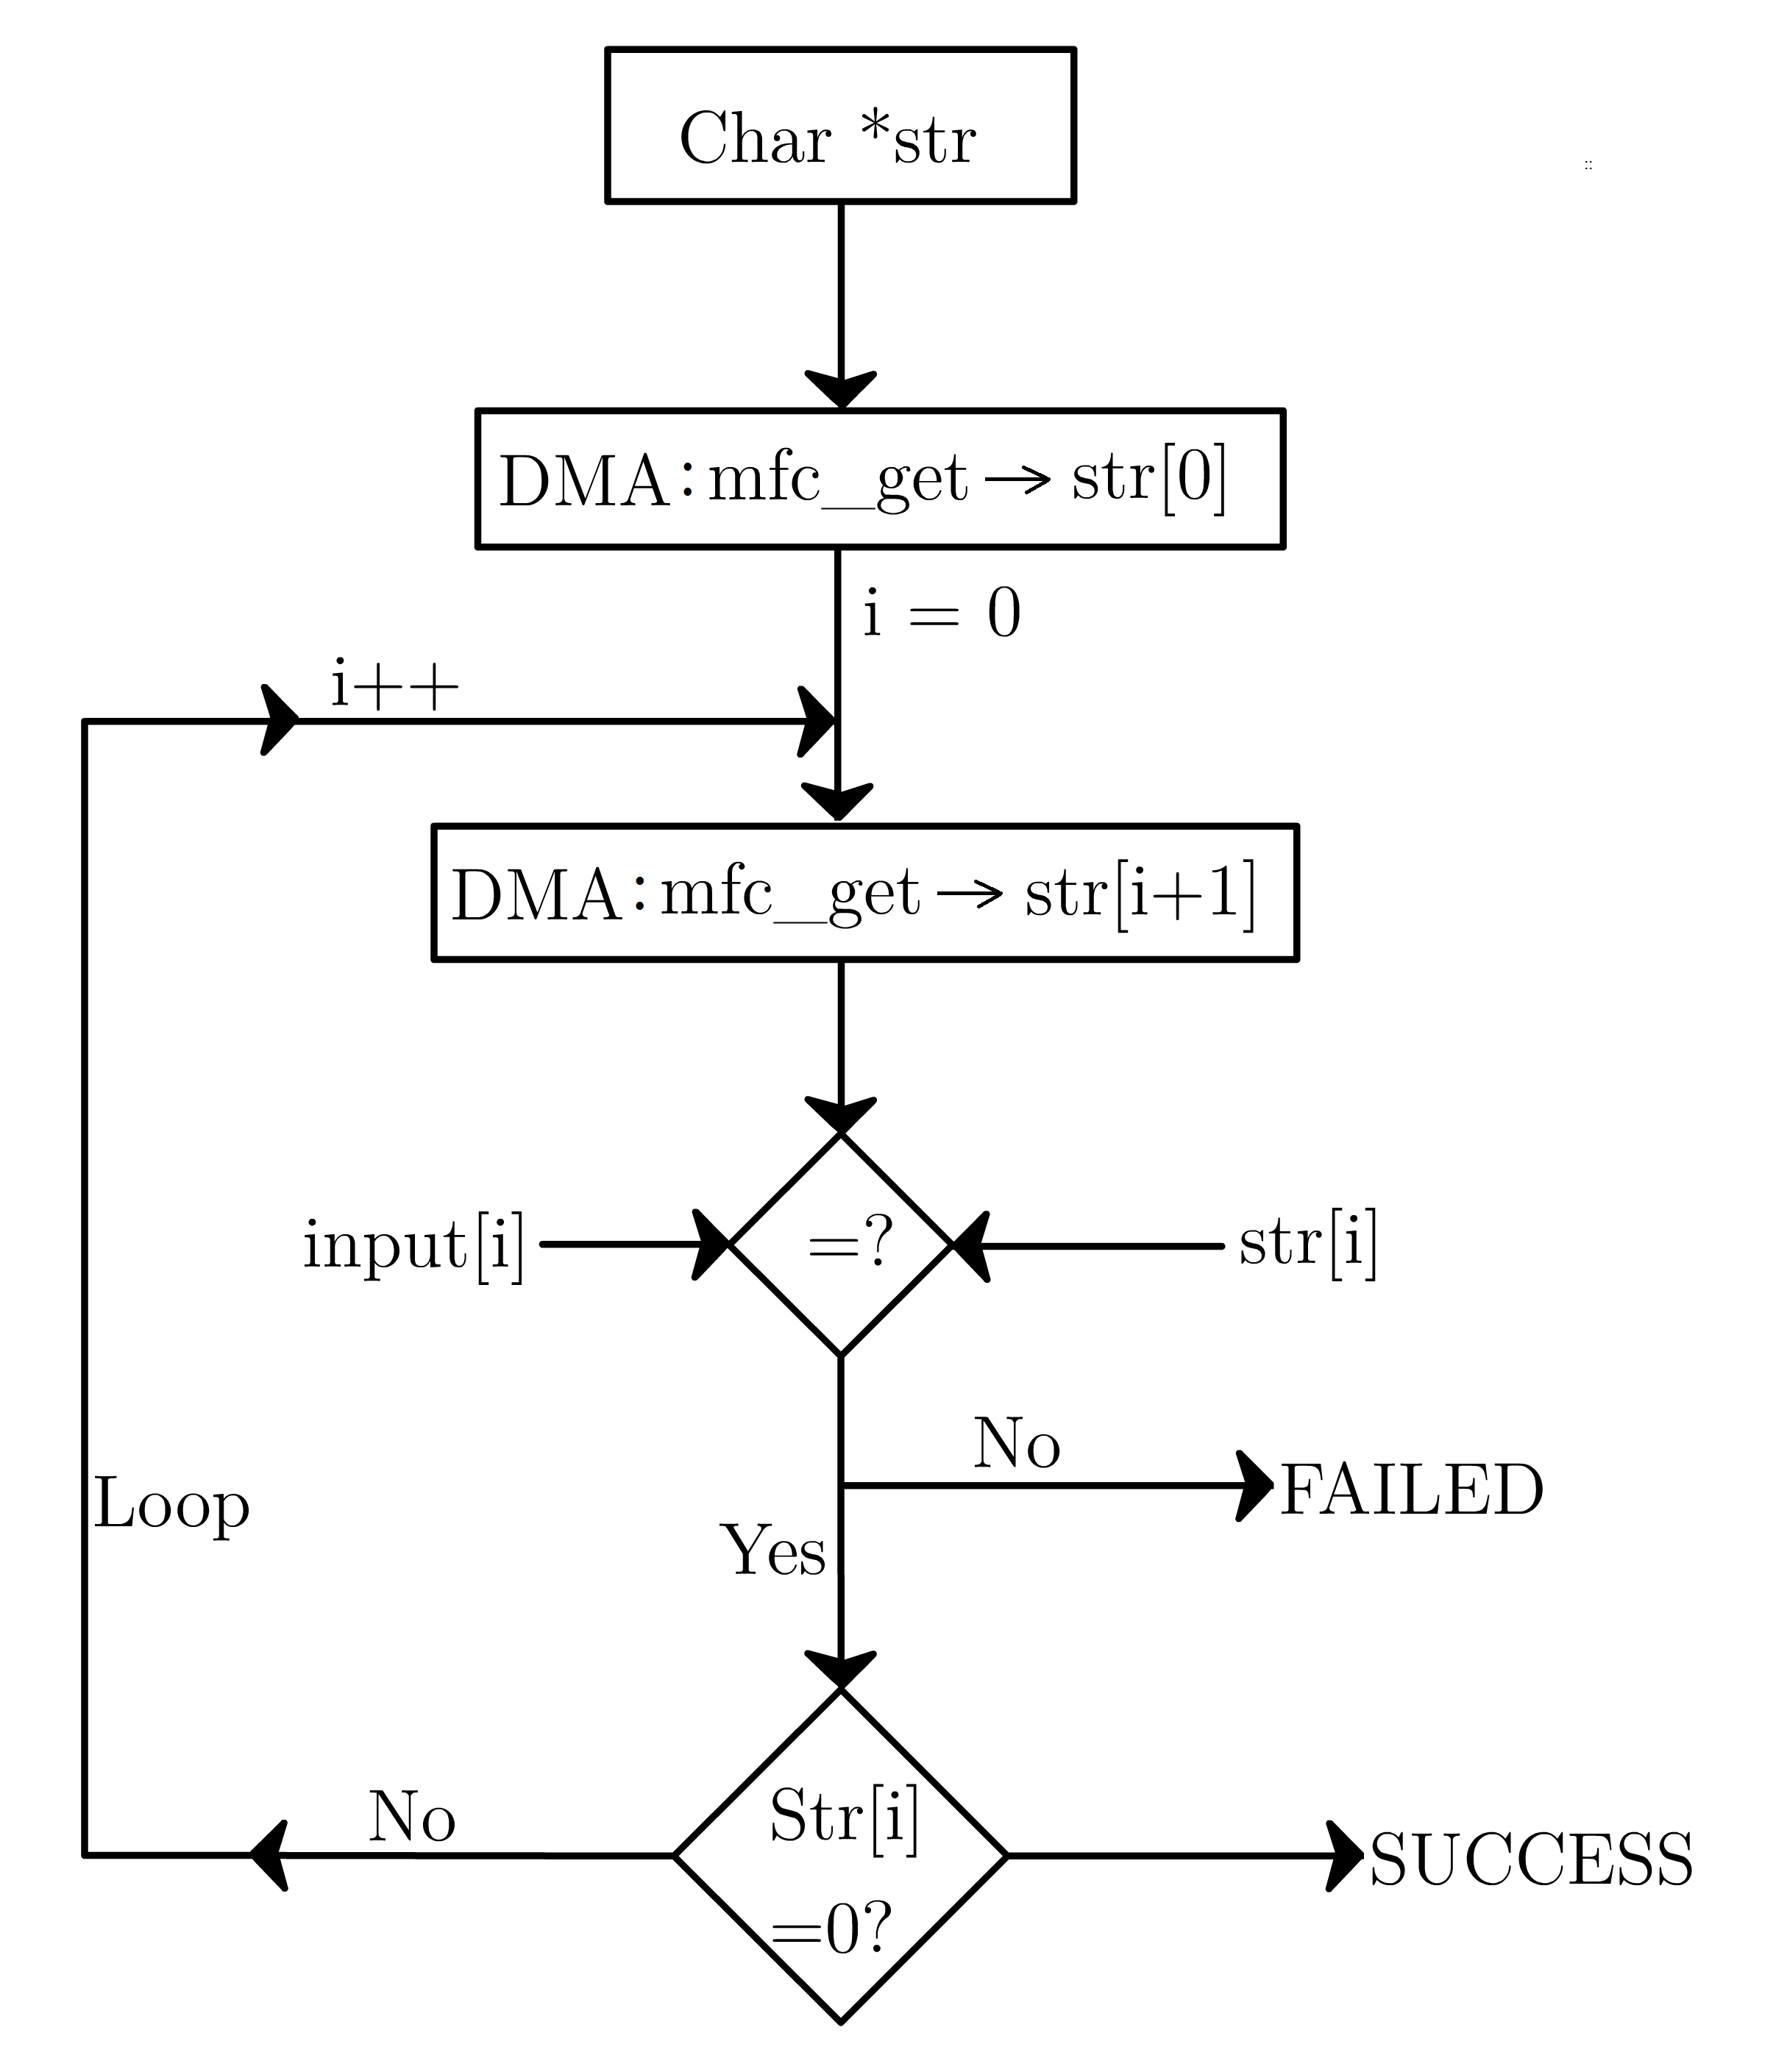
\includegraphics[scale=0.45]{images/DMA.png}}
\caption{DMA double buffering technique for null terminated strings.}
\label{figDMA}
\vspace{-0.03cm}
\end{figure}


\subsection{Results}\label{results}

\begin{figure}
\centerline{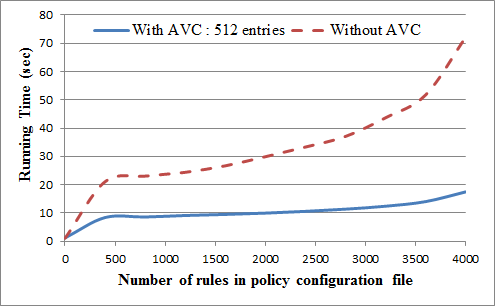
\includegraphics[scale=0.65]{images/rules.png}}
\caption{Single core (PPE) performance of SELinux security context validation}
\label{figGraphRules}
\vspace{-0.01cm}
\end{figure}

Figure \ref{figGraphRules} shows the running time of security context validation measured during the re-labeling process with increasing number of rules in the security policy configuration.
We analyze the difference in the rate of increase of
running time for the two curves. The curve without AVC shows a considerable increase (by about 40\%) in run-time with 
number of rules in the range (0 - 2000], whereas in the same range,
the curve with AVC shows only a negligible increase (by about 8\%) in running time. However when the number of rules is in the range [2500, 4000], the
increase in running time is considerably higher in both cases, which is 64\% and 112\% for with and without AVC respectively. An intuitive explanation for this phenomenon is that the hit ratio of the AVC is generally quite high with fewer number of policy rules. This immense drop in performance in the absence of AVC also establishes the fact that security context validations are computationally intensive. In most modern day systems, the number of
rules in a security policy is well in excess of 5000, hence even with an optimal size of 
AVC, the performance overhead of SELinux is significant.

Figure \ref{figGraphTech} shows a histogram of the running time of different 
techniques with a fixed number of rules (4000) in the security policy. The results show that in the presence of AVC,  the running time of the proposed
SIMD techniques is higher than the single core run-time. This contrasts our intuition that using more cores should generally performance better. Our investigation reveals the cause to be an overhead in SPE due to - 1) initialization, which is the act of loading an executable binary to the SPEs' local cache and 2) data transferred from main memory during execution. We also observe that techniques that use busy-wait strategy perform reasonably better, since the overhead due to repeated initialization is considerably reduced.  For instance, the running
times of $6U$ and $6UBW$ are 38\% and 7\% higher than single core
running time respectively, which goes to show the dominant impact of
SPE initialization on the overall performance.

\begin{figure}
\centerline{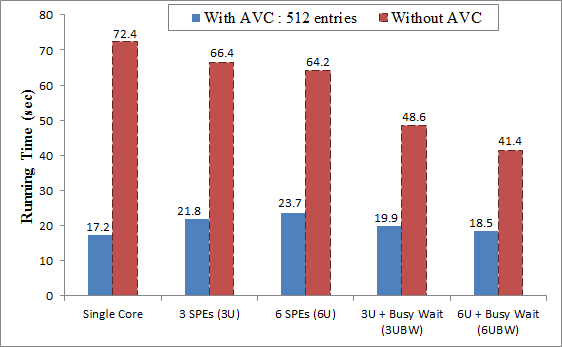
\includegraphics[scale=0.58]{images/techs.png}}
\caption{Comparison of running time of different techniques for SELinux security context validation (with 4000 rules in security policy)}
\label{figGraphTech}
\vspace{-0.05cm}
\end{figure}

The results in the absence of AVC show a stark reversal to those observed earlier. The running time of techniques that use multiple cores is lower than single core run-time.
Although this is as expected, the variation in the efficiency requires
further insights. We observe that the sans busy wait strategies
perform only slightly better than single core, with an efficiency gain of about 8\% and 11\% for $3U$ and $6U$ respectively. On the
other hand, the techniques that use busy wait strategy, considerably
outperform both single core and their SIMD counterparts, with a gain in efficiency of 32\% and 43\% for $3UBW$ and $6UBW$
respectively. Once again the $BW$ strategies show a significant
reduction in run-time since it virtually eliminates the more
prevailing overhead of SPE initialization. Table \ref{tab1} shows the
relative gain / loss in efficiency of each of the proposed techniques when
compared to the single core performance.

\begin{table}[ht]
\centering
\caption{Comparison of relative gain / loss in efficiency of proposed techniques against the single core (PPE) performance.}
\begin{tabular}{|c|c|c|c|c|} \hline
 &\textbf{3U}&\textbf{6U}&\textbf{3UBW}&\textbf{6UBW}\\ \hline
\textbf{With AVC}& -26\%& -38\%& -15\% & -7\%\\ \hline
\textbf{Without AVC}& 8\%& 11\%& 32\% & 43\%\\ \hline
\hline\end{tabular}
\label{tab1}
\end{table}

The key take-away from our results is that, security
validations in general can be modified for parallel executions. But
the gain in efficiency depends on the architecture of the software and
the hardware platform. Our approach can be easily adapted to applications with a similar security validation framework running on other multicore platforms.

\section{Conclusion and Future Work}\label{conclusion}

Although there has been considerable research in the field of software
security, little has been done to improve the delay in
performance that it causes. To deal with the demand of growing
security requirements, modern day operating systems provide
sophisticated in-built security features like the Security Enhanced
Linux (SElinux). These often result in unacceptably low system performance. We hypothesized that security validations in general,
can be optimized by exploiting their inherent data parallelism. We ran several experiments to evaluate the performance of SElinux when modified for concurrent execution. Our experimental setup consisted of automatically generating security policies and measuring the running time involved in SELinux security context validation, on a CBE processor. We obtained contrasting results wherein both gain and loss in efficiency were observed depending on the technique and system configuration. Our investigations revealed that performing computations on the SPE came with a significant overhead in terms of loading time and data transfers. However, we found that the overhead in SPEs can be overcome by utilizing them more often and for longer duration.

\eat{ The performance comparison was made under two
different parameters - the number of rules in the policies and the
presence / absence of AVC in SELinux security server module. Our
results showed that the presence of AVC ensured the performance
overhead was within an acceptable limit, but this did not hold for
policies with a reasonably large number of rules. We also observed
contrasting results with the use of parallel execution techniques, in
fact a loss in performance when compared to single core performance in
the presence of AVC. Whereas a gain in performance of up to 43\% was
measured with one of the multi-processor techniques in the absence of
AVC. Our investigations revealed that Synergistic Processing Element
(SPE) execution had a significant overhead in terms of loading time
and data transfers. However, in the absence of AVC, the SPEs were
utilized more often and long enough to overcome the delay due to
loading and data transfers and thereby register a net gain in
efficiency.}

In general, software applications designed for a uniprocessor system cannot be easily optimized for parallel computing and even when modified the gain in efficiency may not be significant. The problem is prominent in security related applications, since the priority is robustness over efficiency. We believe our work will inspire future research in building applications that harness the potential of multi-core processors. 

One obvious extension of our work is to apply the proposed techniques
to other security features / applications like TOMOYO Linux, SMACK\footnote{http://schaufler-ca.com/}, etc. and compare their performances. Evaluating performance on different
multi-core architectures like GPGPUs, modern PCs and mobile devices
could give greater insights into the effectiveness of the approach
e.g. performance analysis of
\textbf{SEAndroid}\footnote{http://selinuxproject.org/page/SEAndroid},
a MAC mechanism for Android platform.  Another interesting direction could be to analyze
 the proposed techniques in distributed platforms like Beowulf
 clusters and grid networks.
\bibliographystyle{IEEEtran}
\bibliography{references}
\end{document}
